% Informe del proyecto LFIS428 (Grupo 3) con la plantilla de Astronomy & Astrophysics.
% Compilar con pdflatex + bibtex (Overleaf lo hace automáticamente).
\PassOptionsToPackage{spanish,es-noshorthands,english}{babel}
\documentclass{aa}

\usepackage{graphicx}
\usepackage{txfonts}
\usepackage{amsmath}
\usepackage{booktabs}
\usepackage{xcolor}
\usepackage[hidelinks]{hyperref}

\graphicspath{{figuras/}}

\newcommand{\dd}{\mathrm{d}}
\newcommand{\vx}{\mathbf{x}}
\newcommand{\vr}{\mathbf{r}}
\newcommand{\vv}{\mathbf{v}}

\begin{document}
\selectlanguage{spanish}
\nolinenumbers
\renewcommand{\figurename}{Fig.}
\renewcommand{\tablename}{Tabla}
\renewcommand{\refname}{Referencias}

   \title{La ecuación de Poisson comóvil en dos dimensiones}
   \subtitle{Validación de un solver de relajación en CPU y plan de aceleración en GPU}

   \author{C. F. Pincheira Pincheira\inst{1}
        \and [Integrantes del Grupo 3]\inst{1}
        }

   \institute{Instituto de Física y Astronomía, Universidad de Valparaíso,
              Gran Bretaña 1111, Valparaíso, Chile}

   \date{Proyecto del curso LFIS428, Programación en GPU y Optimización, 2026}

  \abstract
   {La formación de estructura en el universo está gobernada por la gravedad actuando sobre pequeñas fluctuaciones de densidad en un fondo en expansión. Las simulaciones cosmológicas de N-cuerpos resuelven en cada paso de tiempo la ecuación de Poisson para el potencial gravitatorio peculiar, lo que hace del solver de Poisson una pieza central de su costo.}
   {Adaptar el código de referencia del curso, que resuelve $\nabla^2u=f$ con condiciones de Dirichlet, a la ecuación de Poisson comóvil en una caja periódica, validarlo y preparar su paso a GPU.}
   {Derivamos la ecuación de Poisson comóvil a partir de la gravedad newtoniana en un fondo de Friedmann. La discretizamos con el laplaciano de cinco puntos y la resolvemos con Jacobi, Gauss-Seidel rojo-negro y SOR rojo-negro, incluyendo la condición de compatibilidad, la fijación del modo cero y el parámetro de sobrerrelajación óptimo para bordes periódicos. Aplicamos el solver a un campo gaussiano aleatorio y a una simulación \emph{particle-mesh} bidimensional.}
   {El error de discretización escala como $h^2$ y el solver alcanza la precisión de máquina. El número de iteraciones sigue la predicción espectral: $\propto N^2$ para Jacobi y $\propto N$ para SOR, con un factor $\sim140$ entre ambos para $N=256$. El espectro del potencial cumple $P_\phi\propto P_\delta/k^4$, y la simulación reproduce el crecimiento lineal $\delta\propto a$, la formación de la red cósmica y la constancia del potencial en un universo de Einstein--de Sitter.}
   {El solver de CPU está validado y su estructura (una función por operación sobre la malla) se traduce directamente en kernels de CUDA. El problema está limitado por el ancho de banda de memoria, lo que orienta las optimizaciones de la siguiente etapa.}

   \keywords{cosmología: teoría -- estructura a gran escala del universo -- métodos: numéricos -- métodos: simulaciones de N-cuerpos}

   \maketitle
   \nolinenumbers

%==========================================================================
\section{Introducción}

El universo temprano era casi perfectamente homogéneo: las fluctuaciones de temperatura del fondo cósmico de microondas son de una parte en $10^5$. Hoy la materia forma una red cósmica de galaxias, cúmulos, filamentos y vacíos. Esa transformación se debe a la gravedad, que amplifica las sobredensidades en competencia con la expansión del universo \citep{Peebles1980,Dodelson2020}.

Mientras el contraste de densidad es pequeño, $\delta\ll1$, la evolución se describe con teoría de perturbaciones lineal \citep{Bernardeau2002}. Cuando $\delta\sim1$ la teoría lineal deja de valer y hay que simular. Un código de N-cuerpos del tipo \emph{particle-mesh} (PM) repite en cada paso: (i) depositar las partículas en una malla para obtener $\delta(\vx)$; (ii) resolver la ecuación de Poisson comóvil para el potencial $\phi$; (iii) calcular la fuerza $-\nabla\phi$; y (iv) mover las partículas \citep{Hockney1988,Bertschinger1998}. Códigos como GADGET-2 \citep{Springel2005} y RAMSES \citep{Teyssier2002} siguen este esquema; las simulaciones en relatividad general como GRAMSES resuelven además varias ecuaciones elípticas del mismo tipo para los potenciales de la métrica \citep{BarreraHinojosa2020a,BarreraHinojosa2020b}. Una revisión reciente del campo se encuentra en \citet{AnguloHahn2022}.

El paso (ii) se repite miles de veces por simulación. Su estructura es ideal para una GPU: la actualización de cada punto de la malla depende solo de sus cuatro vecinos, de modo que millones de puntos se pueden actualizar en paralelo. Este informe documenta la primera etapa del proyecto: la física, la adaptación del código de referencia a la caja cosmológica, su validación y el plan para portarlo a CUDA.

%==========================================================================
\section{Marco teórico}

\subsection{La expansión como gravedad newtoniana}

Consideremos una esfera de radio físico $r=a(t)\,x$ en un universo homogéneo de densidad $\bar\rho(t)$, donde $a(t)$ es el factor de escala y $x$ la coordenada comóvil. Por el teorema de Gauss solo atrae la masa interior, $M=\tfrac{4\pi}{3}\bar\rho\,r^3$:
\begin{equation}
  \ddot r = -\frac{GM}{r^2} = -\frac{4\pi G}{3}\,\bar\rho\,r .
\end{equation}
Con $x$ constante, $\ddot r=\ddot a\,x$, y dividiendo por $a\,x$ obtenemos la ecuación de aceleración de Friedmann para materia,
\begin{equation}
  \frac{\ddot a}{a} = -\frac{4\pi G}{3}\,\bar\rho .
  \label{eq:friedmann}
\end{equation}

\subsection{Ecuación de movimiento comóvil}

Una partícula en el potencial total $\Phi$ cumple $\ddot\vr=-\nabla_r\Phi$. Con $\vr=a\,\vx$,
\begin{equation}
  \ddot\vr = \ddot a\,\vx + 2\dot a\,\dot\vx + a\,\ddot\vx .
\end{equation}
Separamos $\Phi=\Phi_0+\phi$ en la contribución del fondo homogéneo y la de las perturbaciones. El fondo cumple $\nabla_r^2\Phi_0=4\pi G\bar\rho$, con solución $\Phi_0=\tfrac{2\pi G}{3}\bar\rho\,r^2$, y por la Ec.~(\ref{eq:friedmann})
\begin{equation}
  -\nabla_r\Phi_0 = -\frac{4\pi G}{3}\bar\rho\,\vr = \frac{\ddot a}{a}\,\vr = \ddot a\,\vx .
\end{equation}
El fondo genera exactamente la expansión. Igualando las dos expresiones para $\ddot\vr$, los términos $\ddot a\,\vx$ se cancelan; dividiendo por $a$ y usando $\nabla_r=a^{-1}\nabla_x$ y $H=\dot a/a$,
\begin{equation}
  \ddot\vx + 2H\dot\vx = -\frac{1}{a^2}\nabla_x\phi .
  \label{eq:movimiento}
\end{equation}
El término $2H\dot\vx$ es el arrastre de Hubble.

\subsection{La ecuación de Poisson comóvil}

Restando la ecuación de Poisson del fondo de la total, $\nabla_r^2\phi=4\pi G(\rho-\bar\rho)=4\pi G\bar\rho\,\delta$, con $\delta\equiv(\rho-\bar\rho)/\bar\rho$. En derivadas comóviles, $\nabla_r^2=a^{-2}\nabla_x^2$, y con $\bar\rho=\bar\rho_0a^{-3}$ y $4\pi G\bar\rho_0=\tfrac32\Omega_mH_0^2$:
\begin{equation}
  \nabla_x^2\phi = 4\pi G\,a^2\bar\rho\,\delta = \frac32\,\frac{\Omega_mH_0^2}{a}\,\delta .
  \label{eq:poisson}
\end{equation}
Medimos longitudes en unidades del lado $L$ de la caja y el potencial en unidades de $(H_0L)^2$, como en GRAMSES \citep{BarreraHinojosa2020a}: $\tilde\vx=\vx/L$, $\tilde\phi=\phi/(H_0L)^2$. Como $\nabla_x^2=L^{-2}\nabla_{\tilde x}^2$,
\begin{equation}
  \nabla^2\tilde\phi = \frac32\,\frac{\Omega_m}{a}\,\delta ,
  \label{eq:codigo}
\end{equation}
que es el problema $\nabla^2u=f$ del código, con $u=\tilde\phi$ y $f=\tfrac32(\Omega_m/a)\,\delta$.

\subsection{Crecimiento lineal}

En escalas grandes la materia oscura fría se comporta como un fluido sin presión: sus ecuaciones son los dos primeros momentos de la ecuación de Vlasov con dispersión de velocidades nula \citep{Peebles1980,Bernardeau2002}. En coordenadas comóviles, con velocidad peculiar $\vv=a\dot\vx$, y linealizando (descartando los productos $\delta\,\vv$ y $(\vv\cdot\nabla)\vv$):
\begin{equation}
  \dot\delta + \frac1a\nabla\cdot\vv = 0, \qquad
  \dot\vv + H\vv = -\frac1a\nabla\phi .
\end{equation}
Derivando la primera en el tiempo, con $\tfrac{\dd}{\dd t}a^{-1}=-H/a$, usando la divergencia de la segunda, $\nabla\cdot\vv=-a\dot\delta$ y la Ec.~(\ref{eq:poisson}):
\begin{equation}
  \ddot\delta = \frac{2H}{a}\nabla\cdot\vv + \frac{1}{a^2}\nabla^2\phi
  \;\Rightarrow\;
  \ddot\delta + 2H\dot\delta = 4\pi G\bar\rho\,\delta .
  \label{eq:crecimiento}
\end{equation}
En un universo de Einstein--de Sitter, $a\propto t^{2/3}$, $H=2/(3t)$ y $4\pi G\bar\rho=2/(3t^2)$. Con $\delta\propto t^n$ se obtiene $3n^2+n-2=0$, cuyas raíces son $n=2/3$ y $n=-1$. El modo creciente es $\delta\propto a$, y entonces $\phi\propto a^2\bar\rho\,\delta\propto a^2a^{-3}a$ es constante: la densidad crece pero el potencial se congela.

\subsection{Observables}

El potencial determina buena parte de los observables cosmológicos. En Fourier la Ec.~(\ref{eq:poisson}) implica
\begin{equation}
  P_\phi(k) = \left(\frac{3\Omega_mH_0^2}{2a}\right)^2\frac{P_\delta(k)}{k^4}.
  \label{eq:espectro}
\end{equation}
Las velocidades peculiares, $\vv\propto-\nabla\phi$, distorsionan el espacio de redshift \citep{Kaiser1987}; el lensing débil depende de un potencial que cumple una ecuación de Poisson bidimensional sobre el cielo, $\nabla_\theta^2\psi=2\kappa$ \citep{Kaiser1993,Bartelmann2001}, medido por ejemplo por Hyper Suprime-Cam \citep{Aihara2022,Li2022}; y un potencial que varía en el tiempo produce el efecto Sachs--Wolfe integrado \citep{Sachs1967}. Para una caja de $L=100\,h^{-1}$\,Mpc, $H_0L=10^4$\,km\,s$^{-1}$ y $\phi/c^2\sim10^{-5}$: el campo es débil y la gravedad newtoniana es suficiente; las correcciones relativistas son de este orden \citep{BarreraHinojosa2020a,Beordo2025}.

%==========================================================================
\section{Método numérico}

\subsection{Discretización en una caja periódica}

Una caja cosmológica representa un trozo de un universo homogéneo que se repite, así que usamos bordes periódicos en $[0,1)^2$. La malla tiene $N\times N$ puntos $x_i=ih$, con $h=1/N$, y el laplaciano de cinco puntos es
\begin{equation}
  (\nabla_h^2u)_{i,j} = \frac{u_{i+1,j}+u_{i-1,j}+u_{i,j+1}+u_{i,j-1}-4u_{i,j}}{h^2},
\end{equation}
con índices módulo $N$, que aproxima el laplaciano con error $O(h^2)$.

\emph{Compatibilidad.} Al sumar sobre la malla periódica cada $u_{i,j}$ aparece cuatro veces como vecino y $-4$ veces como centro, de modo que $\sum_{i,j}(\nabla_h^2u)_{i,j}=0$ y la ecuación solo tiene solución si $\sum_{i,j}f_{i,j}=0$. Es la ley de Gauss en una caja periódica. Por eso usamos $f=\tfrac32(\Omega_m/a)(\delta-\langle\delta\rangle)$: el promedio corresponde al fondo, ya contenido en la expansión.

\emph{Modo cero.} Si $u$ es solución, $u+C$ también lo es; fijamos $\langle u\rangle=0$.

\subsection{Métodos de relajación}

Despejando el punto central se obtiene la regla de actualización
\begin{equation}
  u_{i,j} \leftarrow \tfrac14\left(u_{i+1,j}+u_{i-1,j}+u_{i,j+1}+u_{i,j-1}-h^2f_{i,j}\right).
  \label{eq:update}
\end{equation}
\emph{Jacobi} usa solo valores de la iteración anterior. \emph{Gauss-Seidel rojo-negro} actualiza primero los puntos con $i+j$ par y luego los impares; cada color depende solo del otro, de modo que es paralelo dentro de cada color, lo que exige $N$ par en la caja periódica. \emph{SOR} sobrerrelaja: $u\leftarrow u+\omega(u^{\rm GS}-u)$ \citep{Press2007}.

Aplicando la Ec.~(\ref{eq:update}) a un modo de Fourier $e_{p,q}$ del error, el factor de contracción de Jacobi es
\begin{equation}
  \mu_{p,q} = \tfrac12\left[\cos(2\pi ph)+\cos(2\pi qh)\right].
\end{equation}
Excluyendo el modo cero, el más lento es $(p,q)=(1,0)$, con $\rho_J=\tfrac12[1+\cos(2\pi h)]=\cos^2(\pi h)\approx1-\pi^2h^2$. El número de iteraciones para reducir el error en un factor $\varepsilon$ es entonces
\begin{equation}
  k_{\rm J} \approx \frac{\ln(1/\varepsilon)}{\pi^2h^2}\propto N^2 .
  \label{eq:kjacobi}
\end{equation}
Gauss-Seidel rojo-negro tiene $\rho_{\rm GS}=\rho_J^2$ y necesita la mitad. Para SOR, $\omega_{\rm opt}=2/(1+\sqrt{1-\rho_J^2})$; usando $1-\cos^4(\pi h)=\sin^2(\pi h)[1+\cos^2(\pi h)]$,
\begin{equation}
  \omega_{\rm opt} = \frac{2}{1+\sin(\pi h)\sqrt{1+\cos^2(\pi h)}},
  \label{eq:omega}
\end{equation}
con lo que el número de iteraciones escala como $N$. Con bordes de Dirichlet, el modo $(1,0)$ no existe y se recupera la fórmula usual $\omega_{\rm opt}=2/(1+\sin\pi h)$. Multigrid reduciría el trabajo total a $O(N^2)$ \citep{Briggs2000}.

\subsection{Estructura del código}

El código \texttt{poisson\_comovil\_cpu.c} mantiene la estructura del código de referencia del curso: arreglos planos en orden \texttt{[y][x]} con índice \texttt{j*N+i}, el tipo \texttt{real} (\texttt{double}) y una función por operación sobre la malla (Tabla~\ref{tab:funciones}). El programa principal lee los parámetros, construye la fuente, repite bloques de 100 iteraciones seguidos del cálculo del residuo relativo $\|f-\nabla_h^2u\|/\|f\|$ hasta que cae bajo la tolerancia, y escribe el campo final en un archivo binario.

\begin{table}
  \caption{Funciones del código y su papel.}
  \label{tab:funciones}
  \centering
  \small
  \begin{tabular}{@{}ll@{}}
    \toprule
    Función & Papel \\
    \midrule
    \texttt{mas}, \texttt{menos}, \texttt{vecinos} & índices periódicos \\
    \texttt{leer\_delta} & lee $\delta$ desde \texttt{delta.bin} \\
    \texttt{iteracion\_jacobi} & una iteración de Jacobi \\
    \texttt{media\_iteracion\_rb} & un color de GS o SOR \\
    \texttt{norma\_residuo} & $\|f-\nabla_h^2u\|$ (reducción) \\
    \texttt{promedio}, \texttt{restar\_promedio} & compatibilidad y modo cero \\
    \texttt{escribir\_salida} & campos $\phi$ y $\delta$ en binario \\
    \bottomrule
  \end{tabular}
\end{table}

Respecto al código de referencia, los cambios son: $h=1/N$ y vecinos con módulo; actualización de todos los puntos; fuente con el promedio restado; resta del promedio de $u$ en cada chequeo; el $\omega$ de la Ec.~(\ref{eq:omega}); y dos modos de entrada, un modo de Fourier con solución exacta para validar y un campo $\delta$ leído desde archivo.

%==========================================================================
\section{Validación}

\subsection{Un modo con solución exacta}

Con $\delta=\cos(2\pi x)\cos(4\pi y)$, el laplaciano discreto actúa sobre cada coseno como $-\tfrac{4}{h^2}\sin^2(kh/2)$, lo que da una solución discreta exacta (que mide el error del solver) y una continua, con autovalor $-4\pi^2(m^2+n^2)$ (que mide el error de discretización). La Fig.~\ref{fig:convergencia} muestra que el error de discretización baja exactamente un factor 4 al duplicar $N$, mientras el del solver permanece en $10^{-13}$.

\begin{figure}
  \centering
  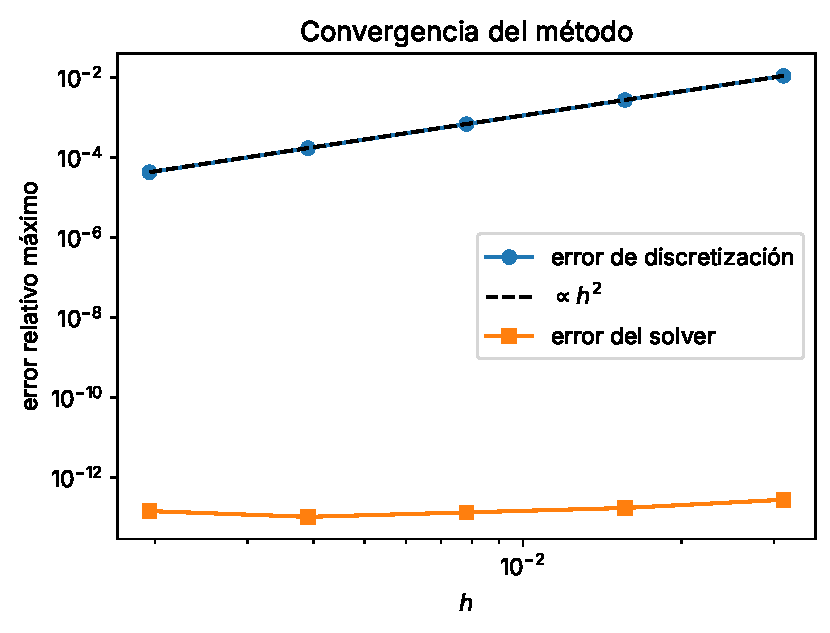
\includegraphics[width=\columnwidth]{convergencia.pdf}
  \caption{Error relativo máximo frente al espaciado $h$. El error de discretización sigue $h^2$; el del solver está en la precisión de máquina.}
  \label{fig:convergencia}
\end{figure}

\subsection{Número de iteraciones}

Con un campo gaussiano aleatorio como fuente, que excita todos los modos, medimos las iteraciones hasta una tolerancia $10^{-8}$ (Tabla~\ref{tab:iteraciones} y Fig.~\ref{fig:iteraciones}). Jacobi sigue la Ec.~(\ref{eq:kjacobi}), Gauss-Seidel necesita la mitad y SOR crece como $N$. Con el $\omega$ de la Ec.~(\ref{eq:omega}), SOR converge en la mitad de iteraciones que con la fórmula de Dirichlet aplicada ingenuamente a la caja periódica.

\begin{table}
  \caption{Iteraciones hasta tolerancia $10^{-8}$ (campo gaussiano).}
  \label{tab:iteraciones}
  \centering
  \begin{tabular}{@{}rrrrr@{}}
    \toprule
    $N$ & Jacobi & Ec.~(\ref{eq:kjacobi}) & GS rojo-negro & SOR \\
    \midrule
    32  & 1\,900   & 1\,911   & 1\,000  & 100 \\
    64  & 7\,200   & 7\,645   & 3\,700  & 200 \\
    128 & 26\,800  & 30\,579  & 13\,700 & 400 \\
    256 & 114\,600 & 122\,317 & 58\,500 & 800 \\
    \bottomrule
  \end{tabular}
\end{table}

\begin{figure}
  \centering
  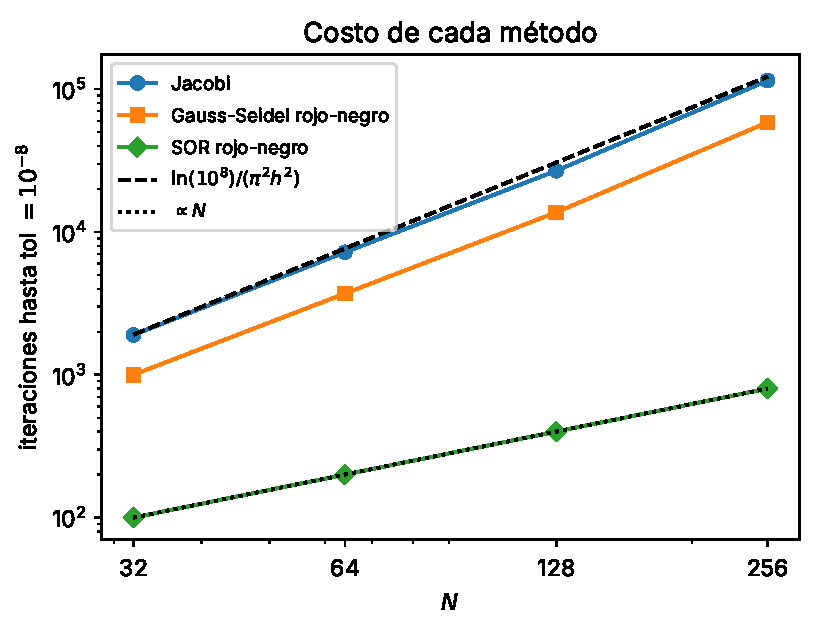
\includegraphics[width=\columnwidth]{iteraciones.pdf}
  \caption{Iteraciones de cada método frente a $N$. La línea discontinua es la Ec.~(\ref{eq:kjacobi}) y la punteada una recta $\propto N$.}
  \label{fig:iteraciones}
\end{figure}

\subsection{Un campo cosmológico}

Para $N=256$ resolvemos con SOR un campo gaussiano con $P_\delta\propto k^{-1}$ y $\sigma_\delta=1$ (Fig.~\ref{fig:campos}). El potencial es mucho más suave que la densidad porque la Ec.~(\ref{eq:poisson}) divide por $k^2$ en Fourier. La diferencia con la solución espectral del mismo problema discreto es $\sim10^{-12}$, y el espectro sigue la Ec.~(\ref{eq:espectro}) (Fig.~\ref{fig:espectros}); en $k$ alto se separa levemente de $k^{-4}$ porque el autovalor discreto, $\tfrac{4}{h^2}\sin^2(kh/2)$, es menor que $k^2$.

\begin{figure}
  \centering
  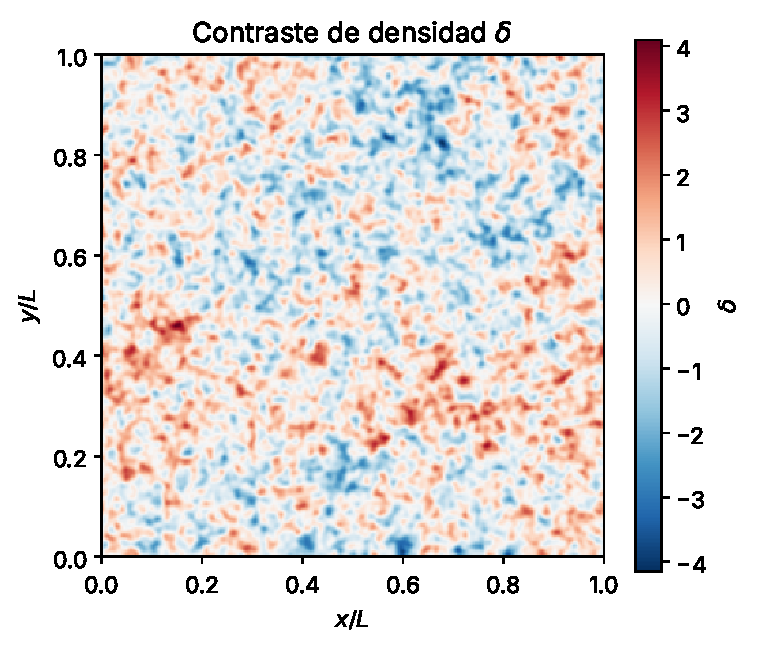
\includegraphics[width=0.49\columnwidth]{delta.pdf}\hfill
  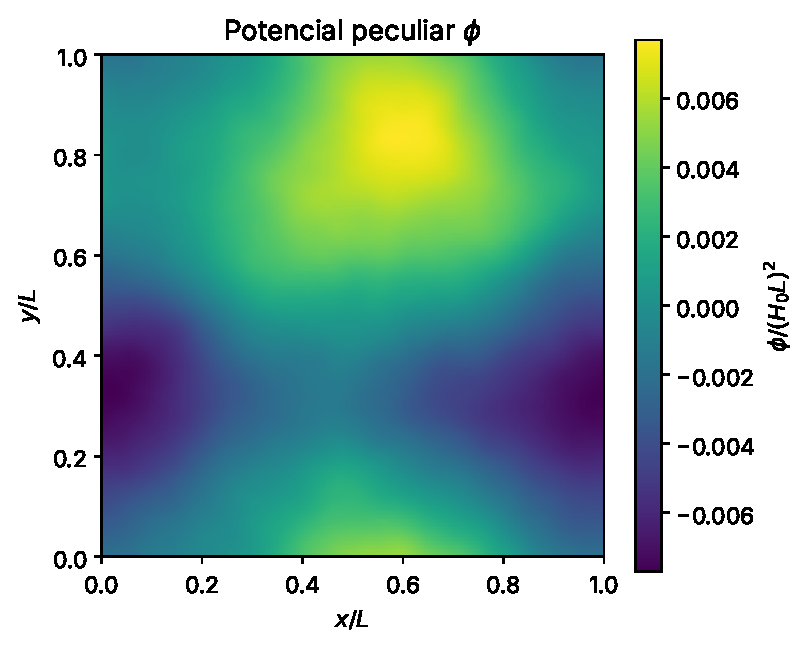
\includegraphics[width=0.49\columnwidth]{potencial.pdf}
  \caption{Izquierda: contraste de densidad $\delta$ de un campo gaussiano. Derecha: potencial peculiar $\tilde\phi$ obtenido con SOR.}
  \label{fig:campos}
\end{figure}

\begin{figure}
  \centering
  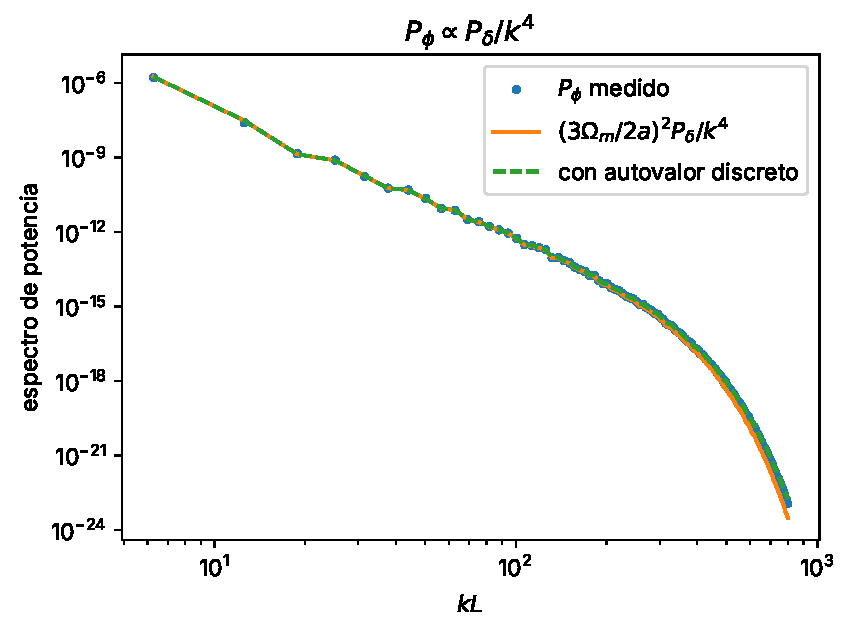
\includegraphics[width=\columnwidth]{espectros.pdf}
  \caption{Espectro del potencial medido frente a la predicción de Poisson continua y discreta.}
  \label{fig:espectros}
\end{figure}

%==========================================================================
\section{Aplicación: simulación particle-mesh bidimensional}

Para mostrar el papel del solver implementamos una simulación PM de juguete con $256^2$ partículas en Einstein--de Sitter. En cada paso se deposita la masa con el esquema \emph{cloud-in-cell}, se resuelve la Ec.~(\ref{eq:codigo}), se calcula la fuerza con diferencias centradas y se integra la Ec.~(\ref{eq:movimiento}) con un esquema leapfrog usando $a$ como variable temporal \citep{Hockney1988,Springel2005}. Las condiciones iniciales usan la aproximación de \citet{Zeldovich1970}: $\vx=\mathbf q+D(a)\boldsymbol\psi(\mathbf q)$, con $\delta=-\nabla\cdot\boldsymbol\psi$ y $D=a$. Es un modelo bidimensional con los coeficientes del caso tridimensional, útil para ilustrar el algoritmo y la física cualitativa.

La Fig.~\ref{fig:pm} muestra la formación de la red cósmica: en $a=0.1$ la distribución es casi uniforme y en $a=1$ hay filamentos, nodos y vacíos. Los filamentos se forman porque el colapso es anisótropo: en la aproximación de Zel'dovich la densidad es $\bar\rho/[(1-D\lambda_1)(1-D\lambda_2)]$ y colapsa primero la dirección del mayor autovalor $\lambda_i$ del tensor de deformación. El potencial, en cambio, casi no cambia, y sus pozos coinciden con las estructuras densas.

\begin{figure*}[t]
  \centering
  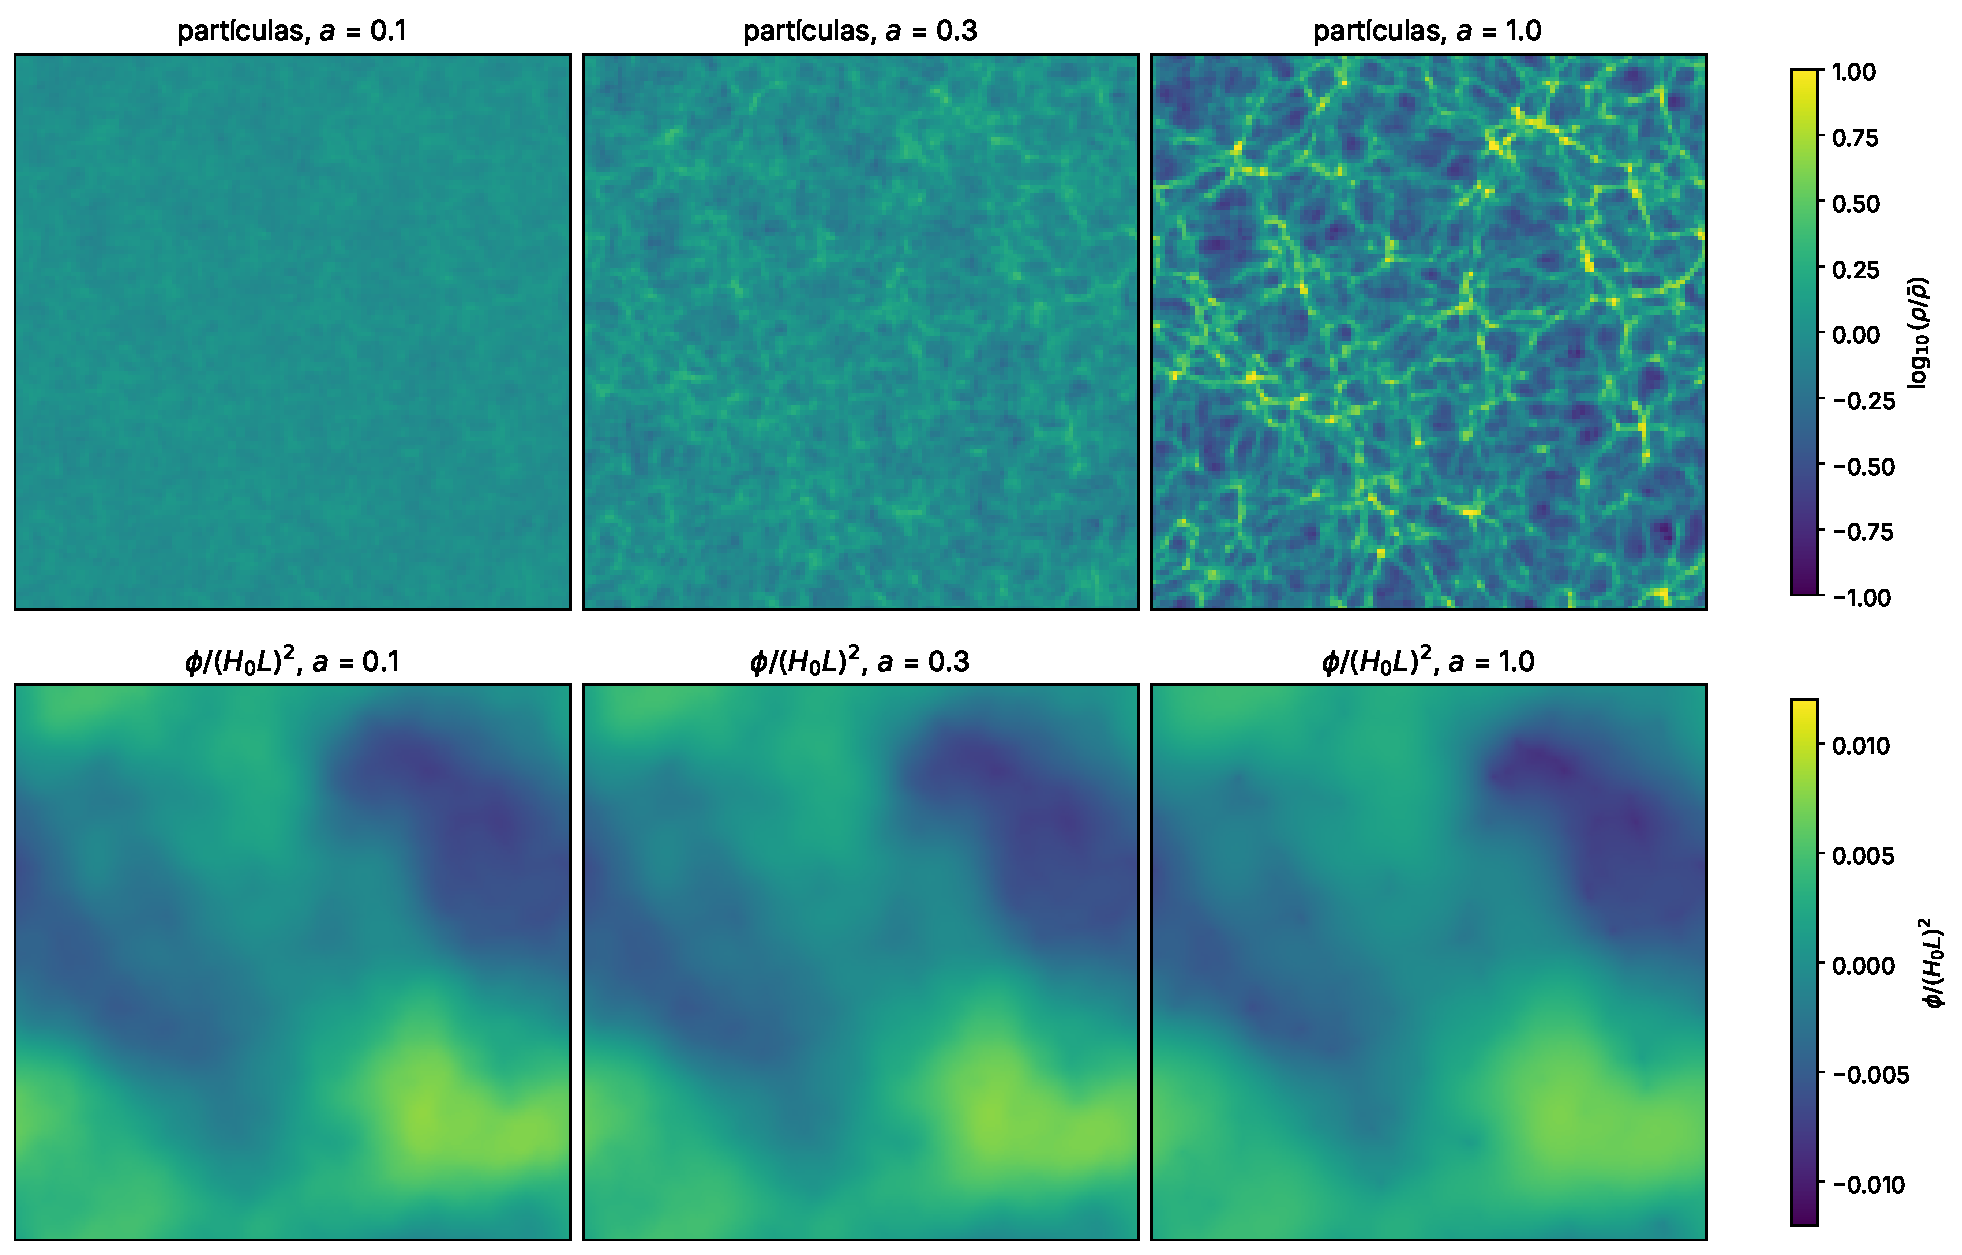
\includegraphics[width=0.92\textwidth]{pm_evolucion.pdf}
  \caption{Simulación PM bidimensional en $a=0.1$, $0.3$ y $1$. Arriba: densidad de partículas, $\log_{10}(\rho/\bar\rho)$. Abajo: potencial peculiar $\tilde\phi$.}
  \label{fig:pm}
\end{figure*}

La Fig.~\ref{fig:crecimiento} cuantifica ambos efectos. La dispersión de la densidad sigue el crecimiento lineal $\delta\propto a$ de la Ec.~(\ref{eq:crecimiento}) hasta $\sigma_\delta\approx0.5$ y luego crece más rápido, en el régimen no lineal. La dispersión del potencial es constante, $\sigma_\phi\approx3.6\times10^{-3}$, incluso en el régimen no lineal, porque $\phi$ está dominado por escalas grandes. Con energía oscura esta curva decaería a bajo redshift, lo que da origen al efecto Sachs--Wolfe integrado \citep{Sachs1967}.

\begin{figure*}
  \centering
  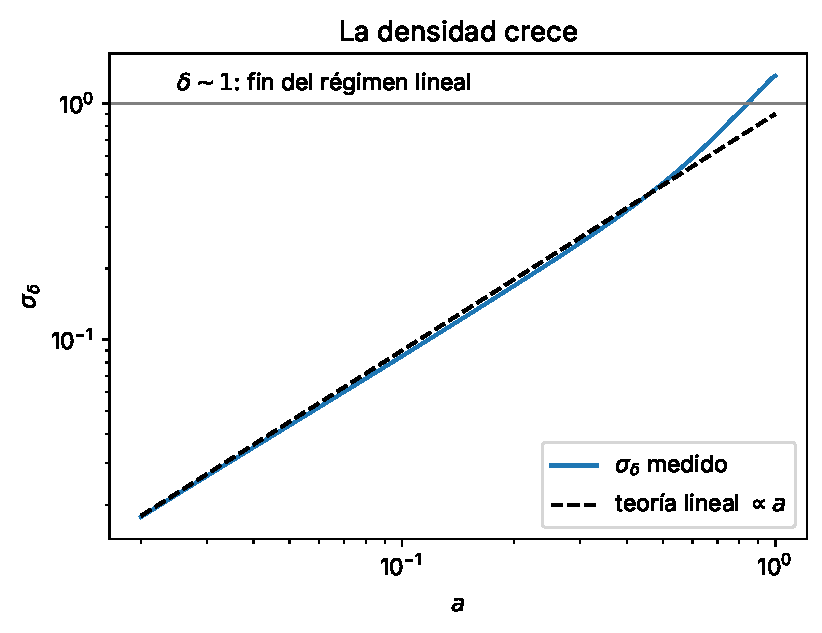
\includegraphics[width=0.46\textwidth]{crecimiento_densidad.pdf}\hfill
  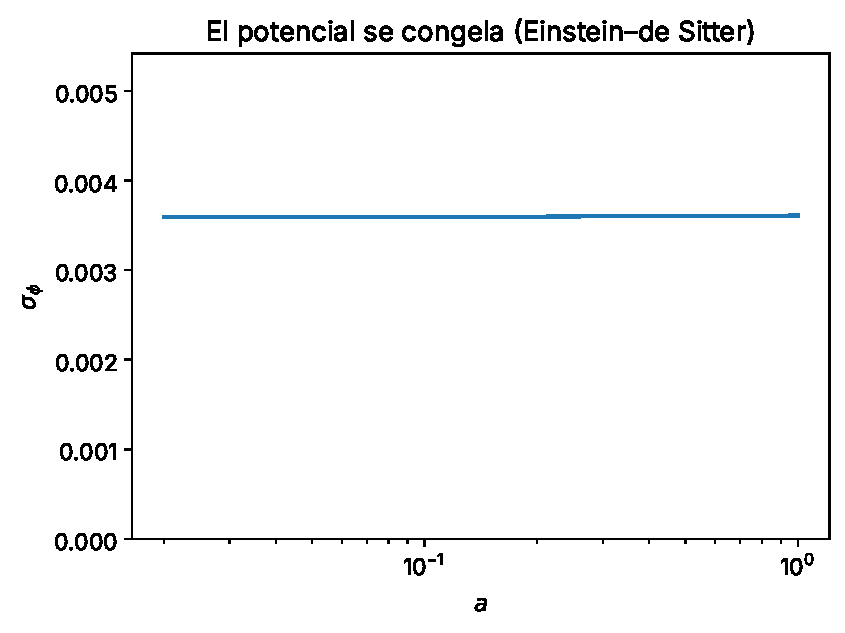
\includegraphics[width=0.46\textwidth]{potencial_congelado.pdf}
  \caption{Izquierda: dispersión de la densidad frente a la predicción lineal $\delta\propto a$. Derecha: dispersión del potencial, constante en Einstein--de Sitter.}
  \label{fig:crecimiento}
\end{figure*}

%==========================================================================
\section{Plan para la GPU}

La versión 1 en CUDA portará cada función de la Tabla~\ref{tab:funciones} a un kernel bidimensional con un \emph{thread} por punto de la malla, con índices periódicos. Los campos $u$, $f$ y $\delta$ se copiarán a la GPU una sola vez al inicio y $u$ volverá al final; en Jacobi se intercambiarán punteros en lugar de copiar datos. El residuo se calculará con una reducción en la GPU, y solo su valor volverá al host cada $M$ iteraciones, para no sincronizar en cada paso.

Cada actualización realiza unas seis operaciones de punto flotante y, con reutilización ideal de datos, mueve tres valores (leer $u$ y $f$, escribir $u$): 24 bytes en doble precisión. La intensidad aritmética es entonces $\sim0.25$ flop/byte, muy por debajo del punto de quiebre del modelo \emph{roofline} de una GPU típica, por lo que el kernel estará limitado por el ancho de banda de memoria. Las optimizaciones candidatas apuntan a reducir el tráfico de memoria: memoria compartida con halo, una reducción eficiente del residuo, fusionar los dos colores en un kernel, precisión simple (justificando la tolerancia alcanzable) y multigrid \citep{Briggs2000}.

%==========================================================================
\section{Conclusiones}

Adaptamos el código de referencia a la ecuación de Poisson comóvil en una caja periódica, con la condición de compatibilidad, el modo cero y el parámetro de sobrerrelajación correcto. La validación confirma el orden $h^2$ del esquema y el número de iteraciones predicho por el análisis espectral, y la aplicación a una simulación PM reproduce la física esperada: crecimiento lineal, formación de filamentos y un potencial congelado. El solver está listo para su paso a GPU, donde su carácter limitado por memoria guiará las optimizaciones.

\begin{acknowledgements}
Agradecemos al profesor C. Barrera-Hinojosa por el código de referencia y la orientación del proyecto.
\end{acknowledgements}

\bibliographystyle{aa}
\bibliography{referencias}

\end{document}
